\documentclass[11pt]{article}
% Shared preamble for the pyMack LST documentation set.
% Used by: mean_boundary_layer.tex, disturbance_equations.tex,
%          numerical_methods.tex, validation.tex
% Each document begins with:  \documentclass[11pt]{article}% Shared preamble for the pyMack LST documentation set.
% Used by: mean_boundary_layer.tex, disturbance_equations.tex,
%          numerical_methods.tex, validation.tex
% Each document begins with:  \documentclass[11pt]{article}% Shared preamble for the pyMack LST documentation set.
% Used by: mean_boundary_layer.tex, disturbance_equations.tex,
%          numerical_methods.tex, validation.tex
% Each document begins with:  \documentclass[11pt]{article}\input{lst_preamble}
\usepackage[margin=1in]{geometry}
\usepackage{amsmath,amssymb,mathtools}
\usepackage{booktabs}
\usepackage{enumitem}
\usepackage{array}
\usepackage{graphicx}
\usepackage{caption}
\usepackage{xcolor}
\usepackage[hidelinks]{hyperref}

\graphicspath{{figures/}}
\captionsetup{font=small,labelfont=bf}

\definecolor{kicol}{RGB}{31,143,107}
\definecolor{boxbg}{RGB}{238,246,242}
\definecolor{rmkbg}{RGB}{244,244,244}

\newcommand{\plain}[1]{\par\smallskip\noindent{\color{kicol}\textbf{In plain words.}}\ \textit{#1}\par\smallskip}
\newcommand{\problembox}[1]{%
  \par\smallskip\noindent\fcolorbox{kicol}{boxbg}{%
  \parbox{0.965\linewidth}{\smallskip\textbf{\color{kicol}What problem is solved here.}\ \ #1\smallskip}}\par\smallskip}
\newcommand{\remark}[2]{%
  \par\smallskip\noindent\colorbox{rmkbg}{%
  \parbox{0.965\linewidth}{\smallskip\footnotesize\textbf{#1}\ \ #2\smallskip}}\par\smallskip}
\newcommand{\bridge}[1]{\par\noindent\textit{#1}\par\medskip}

\newcommand{\D}{\mathrm{D}}
\newcommand{\imag}{\mathrm{i}}
\newcommand{\Real}{\operatorname{Re}}
\newcommand{\Imag}{\operatorname{Im}}
\newcommand{\Mae}{M_e}
\newcommand{\Ree}{\mathit{Re}}
\renewcommand{\bar}[1]{\overline{#1}}
\newcommand{\hatu}{\hat{u}}
\newcommand{\hatv}{\hat{v}}
\newcommand{\hatT}{\hat{T}}
\newcommand{\hatp}{\hat{p}}
\newcommand{\hatq}{\hat{q}}
\newcommand{\nuR}{\nu_{\!R}}

\usepackage[margin=1in]{geometry}
\usepackage{amsmath,amssymb,mathtools}
\usepackage{booktabs}
\usepackage{enumitem}
\usepackage{array}
\usepackage{graphicx}
\usepackage{caption}
\usepackage{xcolor}
\usepackage[hidelinks]{hyperref}

\graphicspath{{figures/}}
\captionsetup{font=small,labelfont=bf}

\definecolor{kicol}{RGB}{31,143,107}
\definecolor{boxbg}{RGB}{238,246,242}
\definecolor{rmkbg}{RGB}{244,244,244}

\newcommand{\plain}[1]{\par\smallskip\noindent{\color{kicol}\textbf{In plain words.}}\ \textit{#1}\par\smallskip}
\newcommand{\problembox}[1]{%
  \par\smallskip\noindent\fcolorbox{kicol}{boxbg}{%
  \parbox{0.965\linewidth}{\smallskip\textbf{\color{kicol}What problem is solved here.}\ \ #1\smallskip}}\par\smallskip}
\newcommand{\remark}[2]{%
  \par\smallskip\noindent\colorbox{rmkbg}{%
  \parbox{0.965\linewidth}{\smallskip\footnotesize\textbf{#1}\ \ #2\smallskip}}\par\smallskip}
\newcommand{\bridge}[1]{\par\noindent\textit{#1}\par\medskip}

\newcommand{\D}{\mathrm{D}}
\newcommand{\imag}{\mathrm{i}}
\newcommand{\Real}{\operatorname{Re}}
\newcommand{\Imag}{\operatorname{Im}}
\newcommand{\Mae}{M_e}
\newcommand{\Ree}{\mathit{Re}}
\renewcommand{\bar}[1]{\overline{#1}}
\newcommand{\hatu}{\hat{u}}
\newcommand{\hatv}{\hat{v}}
\newcommand{\hatT}{\hat{T}}
\newcommand{\hatp}{\hat{p}}
\newcommand{\hatq}{\hat{q}}
\newcommand{\nuR}{\nu_{\!R}}

\usepackage[margin=1in]{geometry}
\usepackage{amsmath,amssymb,mathtools}
\usepackage{booktabs}
\usepackage{enumitem}
\usepackage{array}
\usepackage{graphicx}
\usepackage{caption}
\usepackage{xcolor}
\usepackage[hidelinks]{hyperref}

\graphicspath{{figures/}}
\captionsetup{font=small,labelfont=bf}

\definecolor{kicol}{RGB}{31,143,107}
\definecolor{boxbg}{RGB}{238,246,242}
\definecolor{rmkbg}{RGB}{244,244,244}

\newcommand{\plain}[1]{\par\smallskip\noindent{\color{kicol}\textbf{In plain words.}}\ \textit{#1}\par\smallskip}
\newcommand{\problembox}[1]{%
  \par\smallskip\noindent\fcolorbox{kicol}{boxbg}{%
  \parbox{0.965\linewidth}{\smallskip\textbf{\color{kicol}What problem is solved here.}\ \ #1\smallskip}}\par\smallskip}
\newcommand{\remark}[2]{%
  \par\smallskip\noindent\colorbox{rmkbg}{%
  \parbox{0.965\linewidth}{\smallskip\footnotesize\textbf{#1}\ \ #2\smallskip}}\par\smallskip}
\newcommand{\bridge}[1]{\par\noindent\textit{#1}\par\medskip}

\newcommand{\D}{\mathrm{D}}
\newcommand{\imag}{\mathrm{i}}
\newcommand{\Real}{\operatorname{Re}}
\newcommand{\Imag}{\operatorname{Im}}
\newcommand{\Mae}{M_e}
\newcommand{\Ree}{\mathit{Re}}
\renewcommand{\bar}[1]{\overline{#1}}
\newcommand{\hatu}{\hat{u}}
\newcommand{\hatv}{\hat{v}}
\newcommand{\hatT}{\hat{T}}
\newcommand{\hatp}{\hat{p}}
\newcommand{\hatq}{\hat{q}}
\newcommand{\nuR}{\nu_{\!R}}


\title{\textbf{The Shooting Solver}\\[3pt]
\large Independent verification and refinement of the temporal stability\\
eigenvalue by initial-value integration in \texttt{pyMack}}
\author{\texttt{pyMack} technical documentation}
\date{\today}

\begin{document}
\maketitle
\tableofcontents
\bigskip

%=====================================================================
\section{Scope}\label{sec:scope}
%=====================================================================
The companion numerical-methods document solves the temporal stability problem as a boundary-value
computation: one large matrix pencil, assembled by Chebyshev collocation, handed to a dense
eigensolver that returns all of its eigenvalues at once. The present document poses the identical
question (for a given real wavenumber $\alpha$, at what complex phase speed $c$ does a non-trivial
disturbance satisfy decay at the freestream and the wall conditions?) as an \emph{initial-value}
computation \cite{malik1990}: the disturbance equations are recast as a small first-order system,
integrated from the freestream to the wall, and the eigenvalue is located by driving a $3\times3$
wall matrix singular. No global matrix is ever formed; the cost per evaluation is small, but a good
initial guess is required. This is the classical shooting procedure of Mack \cite{mack1984}, in the
formulation of \"Ozgen \& K{\i}rcal{\i} \cite{ozgen2008}. Within \texttt{pyMack} its role is
verification and refinement: given a mode located by the spectral solver, shooting confirms it
through entirely independent numerics and sharpens it to tight tolerance.

Section~\ref{sec:shoot-system} recasts the disturbance equations as the six-component first-order
system; Section~\ref{sec:shoot-bc} states the wall conditions and constructs the decaying
freestream basis; Section~\ref{sec:shoot-integrate} marches that basis to the wall;
Section~\ref{sec:shoot-wall} converts the wall conditions into the singularity condition on the
wall matrix; Section~\ref{sec:shoot-search} locates the eigenvalue; and
Section~\ref{sec:shoot-compare} places the method against the spectral solver.
Figure~\ref{fig:shooting} shows the complete pipeline.

\paragraph{Notation.} Overbars denote mean (base-flow) quantities; hats denote complex disturbance
amplitudes. $\alpha$ is the real streamwise wavenumber, $c=c_r+\imag c_i$ the complex phase speed,
$\Mae$, $\Ree$, $\mathit{Pr}$, $\gamma$ the edge Mach number, Reynolds number, Prandtl number, and
specific-heat ratio. $Y$ is the six-component shooting state (a $6\times3$ matrix once three
solutions are tracked), $A(y)$ its pointwise $6\times6$ coefficient matrix, $M(c)$ the $3\times3$
wall matrix, and $\sigma_{\min}(c)$ its smallest singular value.

\begin{figure}[H]\centering
  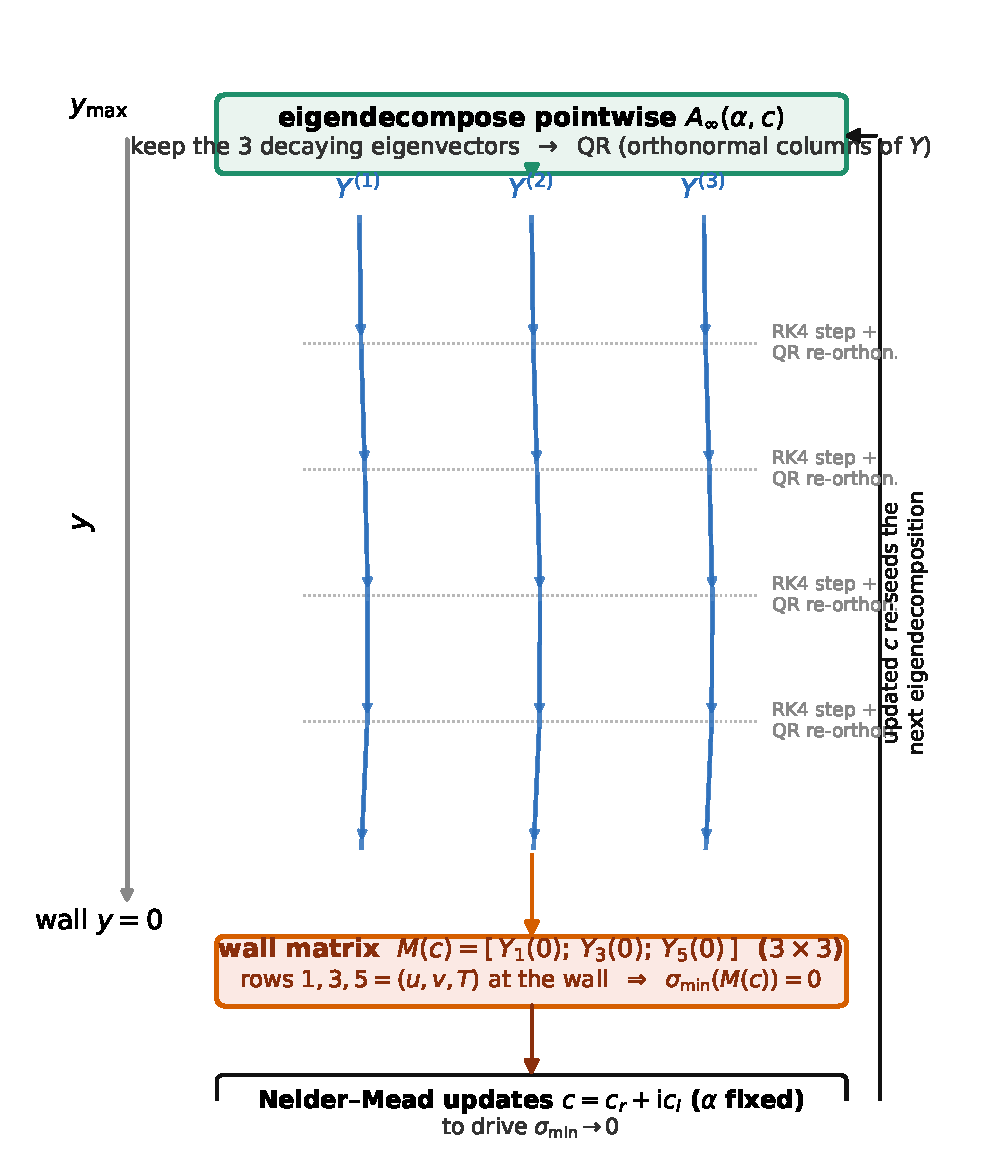
\includegraphics[width=0.78\linewidth]{fig_shooting_scheme.pdf}
  \caption{The shooting pipeline, top ($y_{\max}$) to bottom (wall, $y=0$). At $y_{\max}$ the
  constant-coefficient matrix $A_\infty$ is eigen-decomposed and its three decaying eigenvectors are
  QR-orthonormalised into the starting $6\times3$ basis (Section~\ref{sec:shoot-bc}); the basis is
  RK4-marched to the wall with re-orthonormalisation after every step
  (Section~\ref{sec:shoot-integrate}); at the wall the three arriving columns form the $3\times3$
  matrix $M(c)$ (Section~\ref{sec:shoot-wall}); and an outer Nelder--Mead loop
  (Section~\ref{sec:shoot-search}) updates the trial $c$ to drive $\sigma_{\min}(c)\to0$, feeding
  back into the eigen-decomposition at $y_{\max}$.}\label{fig:shooting}
\end{figure}

%=====================================================================
\section{The first-order state and its coefficient matrix}\label{sec:shoot-system}
%=====================================================================
Given a real wavenumber $\alpha$ and a trial phase speed $c$, the four disturbance equations are cast
as a single first-order ODE in a six-component complex state. Following \"Ozgen \& K{\i}rcal{\i}
\cite[Eqs.~22--28]{ozgen2008}, specialised to two dimensions ($\beta=0$, no spanwise velocity), the
state is
\begin{equation}\label{eq:state}
  Y(y)=\big(X_1,X_2,X_3,X_4,X_5,X_6\big)^{\mathsf T}\in\mathbb C^{6},
\end{equation}
in which $X_1,X_3,X_5$ are the primary flow amplitudes, $X_2,X_6$ the wall-normal derivatives of
$X_1,X_5$, and $X_4$ the pressure amplitude. Concretely, $X_1=\alpha\hatu$ is the wavenumber-scaled
streamwise-velocity amplitude (the $k$-direction combination $\alpha\hat u+\beta\hat w$ of
\cite{ozgen2008} evaluated at $\beta=0$; the constant factor $\alpha$ is immaterial in a homogeneous
eigenvalue problem), $X_3=\hatv$ the wall-normal velocity, $X_5=\hatT$ the temperature (with
$X_2=\D X_1$, $X_6=\D X_5$), and $X_4=\hatp$ the same $\rho_eU_e^2$-scaled pressure as in the
spectral solver, coupled through the continuity and $y$-momentum rows rather than as a plain
derivative. The state thus stacks $(\alpha u,\ \alpha u',\ v,\ p,\ T,\ T')$, and the system closes
as one first-order ODE,
\begin{equation}\label{eq:foode}
  \frac{\mathrm d Y}{\mathrm d y}=A\big(y;\ \alpha,c,\Ree,\Mae\big)\,Y,\qquad A\in\mathbb C^{6\times6},
\end{equation}
where $A$ is assembled \emph{pointwise}, one $6\times6$ matrix at each $y$, from the local
mean-flow data $\bar U,\bar U',\bar U''$, $\bar T,\bar T'$, $\bar\mu$ with
$\mathrm d\mu/\mathrm dT,\ \mathrm d^2\mu/\mathrm dT^2$, and $\bar\kappa$ with its temperature
derivatives. Rows $1$
and $5$ of $A$ carry the trivial derivative definitions $\D X_1=X_2$ and $\D X_5=X_6$ (single
entries $A_{12}=A_{56}=1$); the physics resides in rows $2,4,6$ (the two momentum balances and the
energy balance) and in row $3$, continuity with the equation of state.

The pointwise structure mirrors the block operator of the spectral solver term for term: the
convective factor $\alpha(\bar U-c)$, the viscous prefactor $\propto\Ree/(\bar\mu\bar T)$, the
transport-derivative couplings $\tfrac{\mathrm d\mu}{\mathrm dT}\bar U'$, and the conduction group
in $\bar\kappa$ all reappear, now as scalar entries of a $6\times6$ matrix at one height rather
than as $n\times n$ blocks. The gas defaults ($\gamma=1.4$) and the length scaling ($L^*$) match
the spectral solver, so both routes see the identical mean flow.

\paragraph{Remark: a correction to the printed reference.} The $6\times6$ matrix is evaluated from
the general Appendix-A formulation of Mack \cite{mack1984} at $\beta=0$ with $\lambda/\mu=0$
(the same Stokes closure as the temporal spectral solver), which at those settings is algebraically
identical to the printed Eqs.~22--28 of \cite{ozgen2008}, term for term, with one correction: the
$X_1$ coefficient of the printed Eq.~(24) reads
$+\imag\big(2\mu\tfrac{\mathrm d\mu}{\mathrm dT}T'+\tfrac43\tfrac{T'}{T}\big)$, but re-deriving the
pressure row from Eqs.~(13) and (23) of the same reference gives
$-\imag\big(2\tfrac1\mu\tfrac{\mathrm d\mu}{\mathrm dT}T'+\tfrac43\tfrac{T'}{T}\big)$ (sign and
$\mu$-placement). With the corrected term the two solvers agree in practice: at the reference
parameters of the companion document's worked example ($\Mae=6$, $R=5500$, $\alpha_L=0.174$),
$\sigma_{\min}(c)$ falls to $4\times10^{-6}$ at the spectral eigenvalue $c=0.930+0.0200\imag$ and
rises by two orders of magnitude within $|\Delta c|\sim2\times10^{-3}$ of it.

%=====================================================================
\section{Boundary conditions: the wall and the decaying freestream basis}\label{sec:shoot-bc}
%=====================================================================
Six conditions pin down a non-trivial disturbance: three homogeneous conditions at the wall, and
three at the freestream selecting only the decaying solutions.

\paragraph{Wall conditions.} At $y=0$ the three primary amplitudes vanish,
\begin{equation}\label{eq:wallbc}
  X_1(0)=0\ \text{(no slip)},\qquad X_3(0)=0\ \text{(no penetration)},\qquad
  X_5(0)=0\ \text{(isothermal wall)},
\end{equation}
the pointwise counterparts of the wall identity rows of the spectral assembly.

\paragraph{Freestream: the decaying basis.} As $y\to y_{\max}$ the mean flow becomes uniform and the
coefficient matrix approaches a constant, $A_\infty=A(y_{\max})$. A constant-coefficient system
$\D Y=A_\infty Y$ has solutions $Y\propto e^{\lambda y}v$ built from the eigenpairs $(\lambda,v)$ of
$A_\infty$; the six eigenvalues split into three with $\Real\lambda>0$, which grow outward and are
unphysical, and three with $\Real\lambda<0$, which decay outward as a bounded mode requires. Only the
three decaying eigenvectors are retained,
\begin{equation}\label{eq:decay}
  A_\infty v_k=\lambda_k v_k,\qquad \Real(\lambda_k)<0,\quad k=1,2,3,
\end{equation}
assembled into a $6\times3$ matrix and orthonormalised by a QR factorisation into the starting basis
$Y(y_{\max})$. Enforcing decay in this way is the shooting analogue of the spectral solver's
freestream identity rows. If a trial $c$ yields fewer than three strictly decaying eigenvalues, the
three most decaying (smallest $\Real\lambda$) are taken so the march remains well defined; near
the physical eigenvalue exactly three decay.

%=====================================================================
\section{Integrating the bounded basis to the wall}\label{sec:shoot-integrate}
%=====================================================================
The three admissible freestream solutions must be propagated to the wall so their arrival values can
be tested against \eqref{eq:wallbc}. Because three independent solutions are tracked simultaneously,
the state is the $6\times3$ matrix $Y$ whose columns are the three solutions. It is marched from
$y_{\max}$ down to $y=0$ on a fixed grid of about $800$ steps with the classical
fourth-order Runge--Kutta scheme; over one
step of size $h$ (here $h<0$),
\begin{equation}\label{eq:rk4}
\begin{aligned}
  k_1&=A(y_0)\,Y, & k_2&=A(y_m)\big(Y+\tfrac12 h\,k_1\big), \\
  k_3&=A(y_m)\big(Y+\tfrac12 h\,k_2\big), & k_4&=A(y_1)\big(Y+h\,k_3\big),
\end{aligned}
\qquad
Y\leftarrow Y+\frac{h}{6}\big(k_1+2k_2+2k_3+k_4\big),
\end{equation}
with $y_m=\tfrac12(y_0+y_1)$ the step midpoint and $A(\cdot)$ the pointwise matrix of
Section~\ref{sec:shoot-system}.

\paragraph{Re-orthonormalisation.} The three solutions decay at very different rates, so after a
short march the rapidly decaying columns are numerically swamped by the slowest one and the basis
collapses toward a single direction, the parasitic-error pathology classical in shooting for stiff
stability problems \cite{conte1966,mack1984}. To suppress it, after every RK4 step the columns are
re-orthonormalised by a QR factorisation,
\begin{equation}\label{eq:reortho}
  Y\ \longleftarrow\ Q,\qquad\text{where}\quad Y=QR\ \ (Q\in\mathbb C^{6\times3}\ \text{orthonormal}),
\end{equation}
retaining only the orthonormal factor; the discarded triangular factor merely records scaling. The
operation preserves the \emph{subspace} spanned by the columns while keeping them well conditioned,
and it is that subspace, not the individual column magnitudes, on which the eigenvalue
condition below depends.

%=====================================================================
\section{The eigenvalue condition and the wall matrix}\label{sec:shoot-wall}
%=====================================================================
At the wall the integrated basis is a $6\times3$ matrix $Y(0)$, and any admissible disturbance is a
combination $Y(0)\,a$ of its columns, $a\in\mathbb C^3$. The wall conditions \eqref{eq:wallbc}
require rows $1,3,5$ of that combination to vanish; collecting those rows gives the $3\times3$
\emph{wall matrix}
\begin{equation}\label{eq:wallmat}
  M(c)=\begin{bmatrix} Y_{1}(0)\\ Y_{3}(0)\\ Y_{5}(0)\end{bmatrix}\in\mathbb C^{3\times3},
  \qquad\text{wall conditions:}\quad M(c)\,a=0 .
\end{equation}
A non-trivial $a\neq0$ exists only when $M(c)$ is singular. Rather than testing a determinant, which
is poorly scaled after the repeated re-orthonormalisation, the smallest singular
value of $M(c)$ is monitored,
\begin{equation}\label{eq:sigmamin}
  \sigma_{\min}(c)=\min\operatorname{svd}\!\big(M(c)\big),\qquad
  \boxed{\,\sigma_{\min}(c)\to0\ \Longleftrightarrow\ c\ \text{is an eigenvalue}\,},
\end{equation}
a non-negative, well-scaled measure of distance to singularity: it vanishes exactly when the three
decaying solutions can be combined to satisfy all three wall conditions, that is, exactly when a
genuine boundary-layer mode exists at that $c$.

%=====================================================================
\section{The eigenvalue search}\label{sec:shoot-search}
%=====================================================================
It remains to locate the complex $c=c_r+\imag c_i$ at which $\sigma_{\min}(c)=0$, starting from a
physics-based guess; this single $c$ is the temporal eigenvalue, identical to the one the spectral
solver returns. Since $c$ is complex, driving $\sigma_{\min}\to0$ is a two-dimensional real
minimisation over $(c_r,c_i)$. \texttt{pyMack} applies the Nelder--Mead simplex method
\cite{neldermead1965} to the objective $\sigma_{\min}$, from an initial guess such as the
second-mode estimate $c_r\approx1-1/\Mae$. The search is confined to the physical strip
\begin{equation}\label{eq:bounds}
  c_r\in(0,\,1.2),\qquad c_i\in(-0.2,\,0.2),
\end{equation}
enforced by a large penalty ($10^{6}$) outside the box, and converges to the tolerances
\begin{equation}\label{eq:tols}
  |\Delta c|<10^{-7},\qquad \Delta\sigma_{\min}<10^{-8},
\end{equation}
within at most ${\sim}120$ iterations. Each objective evaluation runs the entire pipeline of
Sections~\ref{sec:shoot-bc}--\ref{sec:shoot-wall} (Figure~\ref{fig:shooting}): build the freestream
decay basis, integrate with re-orthonormalisation to the wall, form $M(c)$, take $\sigma_{\min}$.
The converged minimiser is the eigenvalue, and the growth rate follows exactly as in the spectral
solver, $\omega_i=\alpha c_i$.

%=====================================================================
\section{Spectral versus shooting}\label{sec:shoot-compare}
%=====================================================================
The two solvers answer the identical question (for a given real $\alpha$, at what complex $c$ does
a non-trivial disturbance decay at the freestream and satisfy the wall conditions?) and return the
same physical phase speed, but with complementary characteristics, mirroring the classical
boundary-value/initial-value trade-off \cite{malik1990}:

\begin{center}\small
\renewcommand{\arraystretch}{1.28}
\begin{tabular}{@{}>{\raggedright\arraybackslash}p{3.0cm}>{\raggedright\arraybackslash}p{5.2cm}>{\raggedright\arraybackslash}p{5.2cm}@{}}
\toprule
 & \textbf{Spectral (companion document)} & \textbf{Shooting (this document)} \\
\midrule
core object & one $4n\times4n$ pair $(A,B)$ & one $6\times6$ matrix $A(y)$, evaluated pointwise \\
what it returns & \emph{all} $4n$ eigenvalues at once & \emph{one} eigenvalue near a guess \\
freestream decay & identity rows on the edge nodes & the 3 decaying eigenvectors of $A(y_{\max})$ \\
wall conditions & identity row replacement & $M(c)$ singular, $\sigma_{\min}(c)\to0$ \\
how the answer is found & dense QZ / shift--invert & RK4 march $+$ QR, then Nelder--Mead on $\sigma_{\min}$ \\
initial guess & not required & required (physics-based) \\
memory / cost & large dense matrices, $O((4n)^3)$ & tiny system, cheap per evaluation \\
best used for & surveying the spectrum; sweeping neutral curves and $N$-factors & pinpointing one mode to tight tolerance; independent verification \\
\bottomrule
\end{tabular}
\end{center}

\noindent In practice the two are used together: the spectral solver locates a mode without prior
knowledge of the spectrum, and the shooting solver refines it and confirms it through entirely
independent numerics. Agreement between the two on $c$ is strong evidence that the eigenvalue is
physics rather than a discretisation artifact.

\begin{thebibliography}{99}
\bibitem{mack1984} L.~M. Mack, ``Boundary-layer linear stability theory,'' AGARD Report No.~709,
  \emph{Special Course on Stability and Transition of Laminar Flow}, 1984.
\bibitem{malik1990} M.~R. Malik, ``Numerical methods for hypersonic boundary layer stability,''
  \emph{Journal of Computational Physics}, Vol.~86, No.~2, 1990, pp.~376--413.
\bibitem{ozgen2008} S.~\"Ozgen and S.~A. K{\i}rcal{\i}, ``Linear stability analysis in compressible,
  flat-plate boundary layers,'' \emph{Theoretical and Computational Fluid Dynamics}, Vol.~22, 2008,
  pp.~1--20.
\bibitem{conte1966} S.~D. Conte, ``The numerical solution of linear boundary value problems,''
  \emph{SIAM Review}, Vol.~8, No.~3, 1966, pp.~309--326.
\bibitem{neldermead1965} J.~A. Nelder and R.~Mead, ``A simplex method for function minimization,''
  \emph{The Computer Journal}, Vol.~7, No.~4, 1965, pp.~308--313.
\end{thebibliography}

\end{document}
